\chapter{Conceptual Design}
\label{ch:conceptualDesign}

\section{Requirements}
\label{ch:requirements}

Firstly, the requirements for the synthetic data generation system will be first established.
The goal is to gather a systematic collection of requirements on which the success of the developed system can be measured.
Firstly, non-functional requirements will be explained before continuing with the functional requirements.


\subsection*{Non-Functional Requirements}

Non-functional requirements (or qualitative requirements) describe requirements and constraints on a system that governs how the functions specified in the functional requirements are to be performed \cite{broy2021EinfuehrungSoftwaretechnik}.
They focus on the question of how a system's functional requirements should be realized \cite{broy2021EinfuehrungSoftwaretechnik}.
The ISO-Norm 25010 \cite{SystemsSoftwareEngineering} defined the base characteristics relevant for a software systems quality \cite{haoues2017GuidelineSoftwareArchitecture}.
The key elements of software architecture include functional suitability, reliability, performance efficiency, compatibility, usability, security, maintainability, and portability \cite{haoues2017GuidelineSoftwareArchitecture}.
Each of these is of different importance for each software system.
Additionally, \cite{vogelsang2019RequirementsEngineeringMachine} highlights that additional quality requirements might be necessary in the context of machine learning tasks, for which a standard has yet to be defined.
These could include (but are not limited to) quantitative targets, explainability, freedom from discrimination, legal and regulatory requirements, and data requirements.

This thesis focuses on a research prototype rather than a fully developed software system.
Therefore, only a subset of the abovementioned requirements are prioritized during development.
The following requirements R1 - RN5 are the non-functional requirements for the software developed in this thesis:

%[TODO: GANZER ABSCHNITT AM ENDE AUF INHALTLICHE RICHTIGKEIT KORRIGIEREN]
\begin{description}
    \item[R1 - Functional Suitability:]
    Functional Suitability refers to "the degree to which a product or system provides functions that meet stated and implied needs when used under specified conditions" \cite[p. 219]{bass2013SoftwareArchitecturePractice}.
    In the context of this thesis, the system needs to be able to show how different tabular processing techniques influence the performance of an existing data synthesisation approach.
    This performance should be measured across different similarity measures.

    \item[R2 - Maintainability:]
    Maintainability focuses on the "degree of effectiveness and efficiency with which a product or system can be modified by the intended maintainers" \cite[p. 220]{bass2013SoftwareArchitecturePractice}
    One of the core questions of this thesis is to compare different tabular processing techniques in diffusion models.
    For this, a variety of different approaches are intended to be compared.
    Hence, it is required that the code and software architecture is designed in a maintainable way, such that it can be easily extended with additional processing techniques, not only by the developer, 
    but also for future researchers who might build upon the work of this thesis.

    \item[R3 - Performance efficiency:]
    In the context of deep learning, the program's performance is always essential since training, hyperparameter search and inference usually demand a lot of computation time by nature.
    Consequently, the developed software should reduce unnecessary computations as much as possible.

    \item[R4 - Portability/Reproducibility:]
    Portability is usually referring to the extent of "effectiveness and efficiency with which a system, product, or component can be transferred from one hardware, software, 
    or other operational or usage environment to another" \cite[p. 220]{bass2013SoftwareArchitecturePractice}.
    Since this thesis should encourage other researchers to reproduce and extend the developed codebase, the software should be able to run on other machines running a different operating system given a specified development environment,
    including packages used and their version numbers.
    In general, it is required that all results should be fully reproducible, given the parameters and the configuration of the experiment setups

    \item[R5 - Quantitative Targets:]
    It is required that the different model versions produced in the thesis are compared using metrics that are commonly used in the domain of tabular data synthesis.
    This should enhance the comparability to other approaches.
\end{description}


\subsection*{Functional Requirements}
\label{sec:func_requirements}
Functional requirements describe what the software system should do and which practical aspects must be implemented.
Please note that the software of \cite{kotelnikov2022TabDDPMModellingTabular} will be extended, which has consequences for certain functional requirements.

\begin{description}
    \item[FR1 - Data Import and Export:]
    The software shall support importing tabular data in the same format as specified in \cite{kotelnikov2022TabDDPMModellingTabular},
    where a dataset is separated into numerical, categorical, and target columns, each saved in a NumPy \cite{harris2020array} array. 
    Synthetic data produced by models shall be saved in the same data format.

    \item[FR2 - Tabular Processing:]
    The software shall support tabular data processing techniques that are able to encode and decode tabular data. 
    An \textit{IdentiyProcessor} that has no effect is required to be implemented to test models without any tabular processing mechanism.
    Additional data transformation techniques proposed by \cite{kotelnikov2022TabDDPMModellingTabular}, including normalization or categorical encoding, shall still be supported as intended by the authors.
    Adding new Tabular orocessing mechanisms shall not effect other Tabular processing mechanisms.

    \item[FR2.1 - Tabular processing fit]:
    If necessary, a Tabular processing mechanism should be able to be fitted.
    However, it is required that the tabular processing mechanism only receives training data and does not have access to the test data.

    \item[FR2.2 - Tabular processing transform]:
    Each Tabular processing mechanism needs to transform the raw data into a specified format.

    \item[FR2.3 - Tabular processing inverse transform]:
    Each Tabular processing mechanism needs to able to inverse transformed data back into its original form.

    \item[FR3 - Diffusion Process Configuration]:
    Several experiments with different model configurations will be tested.
    The software shall allow users to configure the diffusion process by specifying parameters such as the number of iterations, batch size, sampling size, and other relevant parameters.

    \item[FR4 - Training, Tuning, Sampling, Evaluation]:
    The software shall support the training of various model versions, including the TabDDPM diffusion model, variations of TabDDPM and other non-diffusion baseline models.
    The module shall allow finding suitable hyperparameters in a specified hyperparameter search space.
    During training, relevant metrics and loss values shall be saved.
    The software shall generate synthetic samples from the trained diffusion model during the sampling process, where the user specifies the number of synthetic samples to be generated.
    The software shall handle the evaluation of synthetic data in multiple ways.
    Firstly, the existing evaluation framework of \cite{kotelnikov2022TabDDPMModellingTabular} shall remain.
    Additionally, a similarity evaluation shall be implemented according to \cite{chundawat2022UniversalMetricRobust}.
    Lastly, the software should also produce visualizations of the synthetic data to allow a visual comparison with the real data.
    
    \item[FR5 - Separation of components:]
    The individual software components (tabular data processing, training, sampling, evaluation) shall be implemented in such a way,
    that they are easy replaceable by alternatives (for tabular data processing) or shall be executed individually (training, sampling, evaluation).
    For example, sampling synthetic data shall be separated from the training so that not every sampling process requires training a model from the start. 
\end{description}


\section{Existing Code Base}
\label{ch:conceptualDesign-existingCodeBase}

The code \cite{akim2023TabDDPMModellingTabular} used in this experiment is based upon the work of \cite{kotelnikov2022TabDDPMModellingTabular}.
It is changed and modified according to the needs of the experiment. 
This section will first explain the architecture of the existing code base before introducing the proposed adaptations in the next section.
An overview of how the overall process in this synthetic data generation approach is done can be seen in \autoref{fig:overall_original}:


\begin{figure}[h]
    \centering
    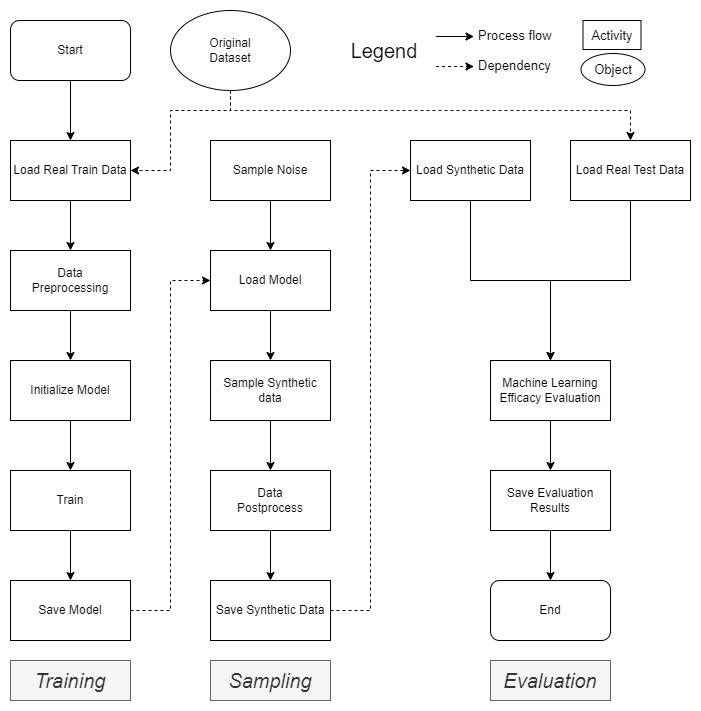
\includegraphics[width=0.8\textwidth]{images/Overall_original.png}
    \caption{Overview synthetic data generation process in \cite{akim2023TabDDPMModellingTabular}}
    \label{fig:overall_original}
\end{figure}


\subsection{Original Implementation}
\label{ch:conceptualDesign-existingCodeBase-originalImplementation}

Kotelnikov \etal provide a software implementation \cite{akim2023TabDDPMModellingTabular} for their proposed TabDDPM.
This implementation consists of multiple scripts and implements several of the functional requirements listed in \autoref{sec:func_requirements}, including FR1, FR4, FR5, and parts of FR4.
This section will explain what kind of software was already provided by \cite{kotelnikov2022TabDDPMModellingTabular} and explain important architectural design choices.

\subsubsection[]{Scripts}
\label{ch:scripts}

The implementation \cite{kotelnikov2022TabDDPMModellingTabular} already provides necessary scripts that allow for an
easy training, sampling, evaluation, and hyperparameter tuning for their proposed TabDDPM model
Additional non-diffusion baseline models the TabDDPM is compared against are supported as well.
The functionality of the most important scripts can be summarized in the following way:

\begin{description}
    \item[train.py:]
    Does the training of the diffusion model.
    Receives configuration parameters for the training.
    It starts by loading the selected dataset and performs preprocessing according to the configuration.
    Afterward, it initializes the required class instances and starts the training loop.
    After the training loop has finished, the trained model and its loss history are saved.

    \item[sample.py:]
    Samples from a pre-trained diffusion model.
    Receives configuration parameters for the sampling process.
    Loads a pre-trained model and samples from the model.
    The new samples are transformed according to the inverse of the preprocessing specified in the configuration.
    After transformation, the generated samples are saved.

    \item[eval\_[catboost|mlp|simple].py:]
    Evaluates a synthetic dataset using machine learning efficacy.
    A machine learning model (specified by the user) is trained on real or synthetic data, specified in the configuration.
    The performance of the model is evaluated on the real test set and metric scores are calculated.

    \item[pipeline\_*.py\footnotemark:]
    Defines the complete pipeline, consisting of training, sampling and evaluation.
    Handles that each function of the pipeline receives the correct attributes from the configuration.
    Allows to execute only specified parts of the pipeline individually.
    \footnotetext[1]{Each implemented baseline model (SMOTE, TVAE, CTABGAN, CTABGAN+) has its own implemention as pipeline\_\textit{modelName}.py}
    
    \item[tune\_*.py\footnotemark:]
    Responsible for the hyperparameter tuning process.
    Starts by defining a hyperparameter search space (see \cite[Table 1, p. 4]{kotelnikov2022TabDDPMModellingTabular} and \cite[Table 7-11, p. 13 f.]{kotelnikov2022TabDDPMModellingTabular})
    Next, an objective function is defined that is maximized for 50 trials through the Optuna framework \cite{optuna_2019}.
    Within the objective function, a set of hyperparameters is selected from the search space.
    With this set of hyperparameters, \textit{pipeline.py} is called to train the model.
    Afterward, for five different random initializations, \textit{pipeline.py} is called to sample and evaluate the model, creating and assessing five different synthetic dataset versions.
    In each training, sampling, and evaluation, the training and validation set are redistributed and shuffled to implement some form of cross-validation \cite{kohavi2001StudyCrossValidationBootstrap}.
    The average evaluation score (machine learning efficacy based) of the five synthetic dataset versions is returned as the objective that Optuna tries to maximize.
    After optimization, the best hyperparameter configuration is saved.
    If specified, a final evaluation of the best found model can be started by calling \textit{eval\_seeds.py}.
    \footnotetext[2]{Each implemented baseline model has its own implementation as tune\_\textit{modelName}.py}
    \item[eval\_seeds.py:]
    Performs an extensive evaluation, given a trained model.
    Starts by loading a pre-trained sampling model ([TabDDPM|SMOTE|CTABGAN|CTABGAN+|TVAE]).
    The script will produce $n_datasets$ synthetic datasets depending on the specified evaluation parameters by calling the sampling script in the respective \textit{pipeline\_*.py} script.
    For each produced dataset, evaluation is performed using a predefined evaluation model ([Catboost|MLP]) for a predefined number of random initializations.
    Ultimately, the average metrics is calculated over all performed runs, reported, and saved.
\end{description}

Hence, to get a fully optimized diffusion model with an extensive evaluation, the user just has to run the \textit{tune\_ddpm.py} script with the \textit{--eval\_seeds} flag.
A detailed activity diagram for each script can be found at \auotref{A:activity_diagrams}.

\subsubsection[]{Configuration}

In order to start one of the above scripts, a configuration file has to be specified, specifying the most important parameters for training, sampling, and evaluation.
For example, \autoref{lst:configuration} shows how such a configuration file could look like and which parameters need to be specified

\begin{lstlisting}[label={lst:configuration}, caption={Example configuration file}]
    parent_dir = "exp/adult/check"
    real_data_path = "data/adult/"
    num_numerical_features = 6
    model_type = "mlp"
    seed = 0
    device = "cuda:0"

    [model_params]
    num_classes = 2
    is_y_cond = true

    [model_params.rtdl_params]
    d_layers = [
        256,
        256,
    ]
    dropout = 0.0

    [diffusion_params]
    num_timesteps = 1000
    gaussian_loss_type = "mse"
    scheduler = "cosine"

    [train.main]
    steps = 1000
    lr = 0.001
    weight_decay = 1e-05
    batch_size = 4096

    [train.T]
    seed = 0
    normalization = "quantile"
    num_nan_policy = "__none__"
    cat_nan_policy = "__none__"
    cat_min_frequency = "__none__"
    cat_encoding = "__none__"
    y_policy = "default"

    [sample]
    num_samples = 216000
    batch_size = 10000
    seed = 0

    [eval.type]
    eval_model = "catboost"
    eval_type = "synthetic"

    [eval.T]
    seed = 0
    normalization = "__none__"
    num_nan_policy = "__none__"
    cat_nan_policy = "__none__"
    cat_min_frequency = "__none__"
    cat_encoding = "__none__"
    y_policy = "default"
\end{lstlisting}    


Model\_type refers to the model that should approximate the noise in the reverse noising process.
Most parameters are self-explanatory, controlling one specific part of the pipeline.
For example, all model\_params specify different relevant aspects for instantiating the model, and diffusion\_params control the diffusion process.
Noteworthy are the train.T and eval.T parameters, which define how preprocessing is done at the beginning of training and evaluation, respectively.
This configuration structure allows to efficiently perform a variety of experiments with different parameters by simply changing the configuration file and inputting it into the next experiment run.

\subsubsection[]{Data format}
\label{sec:data_format}
The authors provide access to 12 different datasets, which have been cleaned and formatted by a program provided by \cite{gorishniy2023EmbeddingsNumericalFeatures}.
Each dataset contains data separated into multiple subparts.
Firstly, the columns are split into categorical, numerical, and target ("y") columns.
Secondly, the datasets are distributed into a training, validation, and testing set.
Therefore, each dataset is separated into nine parts, following the following naming convention:
X\_[cat|num]\_[train|val|test].npy and for the target y\_[train|val|test].npy

Additionally, a \textit{info.json} file is provided, containing the necessary information for handling the data.
In \autoref{lst:info}, one can see how such an info-file contains the information on how the splits mentioned above have been done and what kind of task this dataset usually has (it is differentiated between binary classification (binclass), multiclass classification (multiclass) and regression (regression)).
\begin{lstlisting}[label={lst:info},caption={Example data info file}]
    {
    "name": "Adult",
    "id": "adult--default",
    "task_type": "binclass",
    "n_num_features": 6,
    "n_cat_features": 8,
    "test_size": 16281,
    "train_size": 26048,
    "val_size": 6513
    }
\end{lstlisting}
Inside the code of TabDDPM \cite{akim2023TabDDPMModellingTabular}, a custom dataset class provided by the author handles any dataset that follows the above naming convention and provides a matching information file.

\section{Proposed Concept}
\label{ch:conceptualDesign-changes}

Changes to the current architecture have been made to answer the research questions specified in \auotref{ch:intro-goals}.
\autoref{fig:Overall_changed} shows that the overall synthesisation process does not deviate much from \autoref{fig:Overall_original}.
Changes are highlighted in green and affect each step in the diffusion process, the training, sampling, and evaluation step.
For a detailed overview of how each individual scripts changed, please refer to \auotref{A:activity_diagrams}.

\begin{figure}[h]
    \centering
    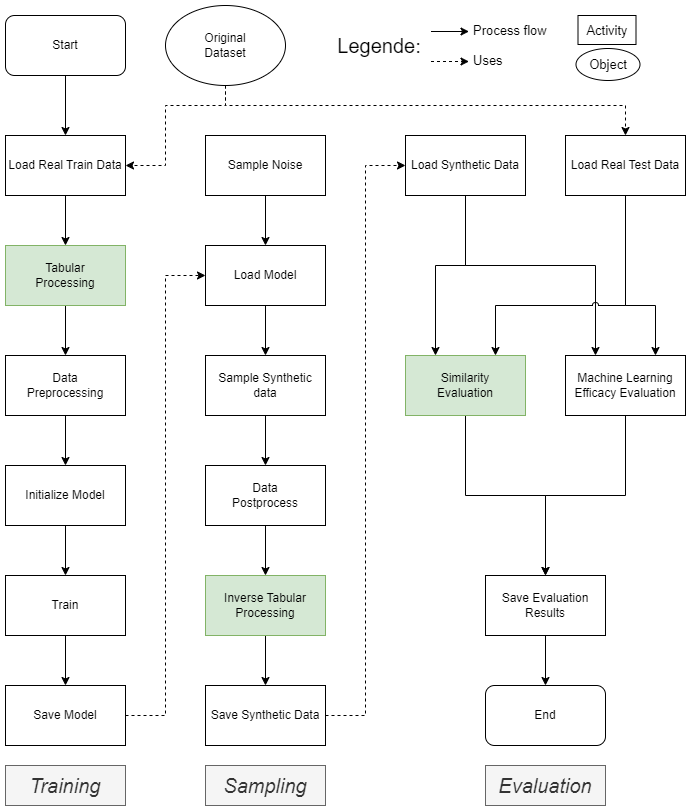
\includegraphics[width=0.8\textwidth]{images/Overall_changed.png}
    \caption{Overview of proposed synthetic data generation process changes (highlighted in green)}
    \label{fig:Overall_changed}
\end{figure}

\begin{description}
    \item[C1-Tabular Processing:] To test the effect of different tabular processing techniques, a "Tabular processing" step is required before training the diffusion model.
    Within this processing, the raw data is transformed according to the defined tabular processing strategy.
    The tabular processing data output format needs to be the same as before the transformation, described in \autoref{sec:data_format}, to ensure 
    that the remaining pipeline remains functional and keeps changes to the original code minimal.
    \item[C2-Inverse Tabular Processing:] Similar to the data preprocessing, which requires an inverse data postprocessing, to turn the data back into its original format and scale, the same is necessary for the tabular processing.
    Since the model is trained on data that has been transformed according to the tabular processing mechanism, the diffusion model will produce data in the same format.
    Consequently, the synthetic data must be transformed by an inverse function of the tabular processing mechanism before the evaluation.
    \item[C3-Similarity Evaluation:] Lastly, an extended evaluation of the synthetic data's similarity to the real data should be performed.
    For this, the original machine learning efficacy evaluation remained unchanged.
    However, the evaluation pipeline is extended by a similarity Evaluation that does not only calculate a unified score, TabSynDex \cite{chundawat2022UniversalMetricRobust}, but also reports other metric results that are of interest.
    Hyperparameters of the generation models can also be tuned towards the TabSynDex score.
    In addition to the numeric metric results, several visualizations comparing real and synthetic data will be generated.
\end{description}

%<-------------
\subsection{Tabular Processing Criteria}
\label{ch:Concept-criteria}

The main source for finding the processing mechanisms should be academic literature, where said mechanism has been applied to a related problem successful
The selection of which tabular processing mechanisms are realized heavily depends on the requirements defined in \autoref{sec:func_requirements}.

For a tabular processing mechanism to be used, the following conditions must be met:

\begin{enumerate}
    \item reversibility: the tabular processing mechanism must not only transform the data into a different format, but it also must be able to revert the transformation
    such that the data can be transformed back into its original form.
    \item compatibility: the data must be able to be separated into numerical and categorical parts after the transformation
    since the remaining code expects data in this format, as specified in \autoref{sec:data_format}.
    \item complexity: the time it takes to transform the data should be within a reasonable timeframe. They shall not add too much computation time to the already extensive model-tuning process.
    \item availability: due to the limited time frame of this thesis, the code for the mechanisms should be publicly available (or could be implemented within a reasonable timeframe).
\end{enumerate}

Based on the criteria mentioned above, tabular processing mechanisms should be selected.


\subsection[]{Evaluation}
\label{ch:conceptualDesign-Evaluation}
The evaluation framework shall contain multiple evaluation aspects.
Firstly, the existing machine learning efficacy using a CatBoost model proposed by \cite{kotelnikov2022TabDDPMModellingTabular} shall be executed and remain untouched.
In addition, the TabSynDex \cite{chundawat2022UniversalMetricRobust} similarity will be performed in each evaluation.
Machine learning efficacy that is based upon an \gls{mlp} or using a set of classification models will not be performed for the following reasons:
\begin{enumerate}
    \item \cite{kotelnikov2022TabDDPMModellingTabular} argues convincingly that machine learning efficacy not based on CatBoost is less informative compared to the CatBoost counterpart.
    \item The TabSynDex metric contains a machine learning efficacy metric based upon a set of models.
\end{enumerate}
Consequently, machine learning efficacy will be evaluated twice in each evaluation, once based on CatBoost and once inside the TabSynDex metric using a set of standard machine learning models.

Lastly, for a visual evaluation, several plots indicating the similarity of the synthetic data to the real data shall be generated using the implementation of \cite{brenninkmeijer2019GenerationEvaluationTabular}.
If necessary, modifications to the plots may be required.

% ''TODO:
% ML efficacy like in the original paper + Tabsyndex similarity score + similarity score of anderes paper (+bilder von denen)

% aufzählen was alles klassische ml efficacy is (acc, f1, roc) und was sim_score werte sind''